% 6 pages max
\documentclass[twocolumn]{article}
% packages
%\usepackage[utf8]{vietnam}
\usepackage{amsmath, amssymb, amsthm}
\usepackage{color, graphicx, cases}
\usepackage{hyperref}
\hypersetup{
	colorlinks=true,
	linkcolor=blue,
	filecolor=blue,      
	urlcolor=blue,
}
\usepackage{array, multirow, booktabs}
\usepackage{caption, subcaption}
\usepackage{ragged2e} % using justifying
\numberwithin{equation}{section}
\everymath{\displaystyle}
\usepackage{titling}
\usepackage{abstract}

\topmargin=-10mm \headsep=5mm \evensidemargin=-12mm
\oddsidemargin=-6mm \textwidth=170mm \textheight=242mm
\columnsep=6mm

%\usepackage[a4paper,left=35mm,top=31mm,right=20mm,bottom=30mm]{geometry}
%\renewcommand{\baselinestretch}{1.5}

% new definitions
\newtheorem{dl}{Theorem}[section]
\newtheorem{md}{Proposition}[section]
\newtheorem{hq}{Corollary}[section]
\newtheorem{cy}{Remark}[section]

\theoremstyle{definition}
\newtheorem{dn}{Definition}[section]
\newtheorem{vd}{Example}[section]
\newtheorem{bt}{Problem}[section]
\newtheorem{nx}{Comment}[section]

% reference
\usepackage{cleveref}
\crefname{dl}{\textbf{Theorem}}{}
\crefname{md}{\textbf{Proposition}}{}
\crefname{hq}{\textbf{Corollary}}{}

\crefname{dn}{\textbf{Definition}}{}
\crefname{vd}{\textbf{Example}}{}
\crefname{cy}{\textbf{Remark}}{}
\crefname{bt}{\textbf{Problems}}{}
\crefname{nx}{\textbf{Comment}}{}

\title{\bf Numerical simulation of heat transfer problem by Freefem++ software}
\author{\normalsize\bf Mai Ta$^{1,2}$, Franck Pigeonneau and Pierre Saramito$^2$}
\date{\normalsize\vspace{-2ex}\em
$^1$~Surface du verre et interfaces, UMR 125 CNRS/Saint-Gobain\\
39, quai Lucien Lefranc - BP 135, 93303 Aubervilliers cedex, France\\
\href{mailto:Franck.Pigeonneau@saint-gobain.com}{Franck.Pigeonneau@saint-gobain.com},\\[1.1mm]
%
$^2$~Lab. J. Kuntzmann, CNRS and Grenoble university\\
51, rue des math\'ematiques BP 53 - Domaine Universitaire, 38041 Grenoble Cedex 9, France \\
\href{mailto:tathithanhmai@gmail.com}{tathithanhmai@gmail.com},
\href{mailto:Pierre.Saramito@imag.fr}{Pierre.Saramito@imag.fr}
}

\justifying
% ---------------------------------------------
\begin{document}
\twocolumn[
\begin{@twocolumnfalse}
\maketitle
\rule{\textwidth}{.1pt}
Abstract\\
\noindent
...
\\
\vspace{1ex}
\noindent {\em Keywords: Inverse source problems, least squares method, Tikhonov regularization, space-time finite element method, conjugate gradient method}
\rule{\textwidth}{.1pt}
\vspace{2mm}
\end{@twocolumnfalse}]

% --------------------------------------------------------------------
\section{Introduction}
% --------------------------------------------------------------------

Let $\Omega \subset \mathbb{R}^d,\, d\in \mathbb{N^+}$ be a bounded domain with a boundary $\Gamma$ and endow the cylinder $Q=\Omega\times (0,\, T]$ and lateral surface area $S=\Gamma \times (0,\, T]$ where $T>0$. 
\\
Consider the heat equation:
\begin{align}\label{1.1}
	\frac{\partial u(x, t)}{\partial t}+\mathcal{L}u(x, t)=F(x, t), \quad(x, t)\in Q,
\end{align}
with the Dirichlet boundary and initial conditions, respectively
\begin{align}
	u(x, t)&=u_D(x, t),\quad(x, t)\in S, \label{1.2}\\
	u(x, 0)&=u_0(x),\quad\quad\, x\in \Omega,\label{1.3}
\end{align}
where
\begin{align*}
	&\mathcal{L}u = -\sum_{i, j=1}^{d}\frac{\partial}{\partial x_i}\left(a_{ji}\frac{\partial u}{\partial x_j}\right)+a_0u,\\
	&a_{ji}\in L^{\infty}(Q),\, a_{ij}=a_{ji},\; \forall i, j\in \{1, 2, ..., d\},\\
	&\lambda_1\left\|\xi\right\|^2\leq \sum_{i, j=1}^{d}a_{ij}\xi_i\xi_j\leq \lambda_2\left\|\xi\right\|^2,\; \forall \xi\in\mathbb{R}^d,\\
	&a_0\in L^{\infty}(Q),\; 0\leq a_0(x, t)\leq \mu_1,\; (x, t)\in Q,\\ 
	&u_0\in L^2(\Omega),\;u_D\in L^2(S),
\end{align*}
with $\lambda_1$ and $\lambda_2$ are positive constants and $\mu_1\geq 0$.
\\
The problem is that to determine $u$ when all data $a_{ji},\,a_0,\,u_0,\,u_D$ and $F$ in \eqref{1.1} - \eqref{1.2} - \eqref{1.3} are given called \textbf{\textit{direct problem}}. But in practice, we miss one of the data above such as  the right hand side $F$ of \eqref{1.1} known for heat source. The problem identifying $F$ when some additional observations on the solution $u$ available called \textbf{\textit{inverse problem}}. We suppose that the heat source following the form $F(x, t)=f(x, t)q(x, t)+g(x, t)$, where $q(x, t),\, g(x, t)$ are given. Find $f(x, t)$ if $\omega(x, t)=u(x, t)$ is given on $Q$. 
% --------------------------------------------------------------------
\section{Numerical method} 
% --------------------------------------------------------------------
\subsection{Direct problem}
% --------------------------------------------------------------------

Find $u(.,t)\in H^1(\Omega)$ such that
\begin{align}\label{2.1}
	\left\langle \frac{\partial u}{\partial t}, v \right\rangle+a\left(u, v\right)=\left\langle F, v \right\rangle,\; \forall v\in H^1(\Omega),
\end{align} 
\begin{align}\label{2.2}
	u(x, 0)=u_0(x), \; x\in \Omega,
\end{align}
where 
$$a\left(u, v\right)=\int_{\Omega}\left[\sum_{i, j=1}^{d}a_{ji}\frac{\partial u}{\partial x_i}\frac{\partial v}{\partial x_j}+a_0uv\right]dx,$$
$$\left\langle \varphi, v \right\rangle=\int_{\Omega}\varphi vdx.$$
Now we present a fully discrete finite element approximation for the variational problem \eqref{2.1} by the Crank-Nicolson method as follows:
\\
For \textit{spatial approximation}, let $\mathcal{T}_h$ be a triangulation of $\Omega$ and define a piecewise linear finite element space $V_h \subset H^1(\Omega)$ by
$$V_h=\left\{v_h:v_h\in C(\overline{\Omega}), v_h|_K\in P_1(K), \forall K\in \mathcal{T}_h\right\},$$
where $P_1(K)$ is a continuous piecewise linear polynomial on the element $K$. 
\\
For \textit{temporal discretization}, discrete $[0, T]$ uniformly into $M$ steps, $t_n=n\Delta t,\, n=0, 1, \dots, M$ with the time step size $\Delta t = T/M$. We define a function $\varphi(x, t)$ and $\varphi(x, t_n)=\varphi^n(x)$.
\\
Find $u^n_h\in V_h$ for $n=1, 2, \dots, M$ such that
\begin{align}\label{2.3}
	\langle d_tu^n_h, v_h \rangle+a\left(\frac{u^n_h+u^{n-1}_h}{2}, v_h\right)=\left\langle \frac{F^n+F^{n-1}}{2}, v_h \right\rangle,
\end{align}
and the initial condition 
\begin{align}\label{2.4}
	u^0_h=u_0,
\end{align}
where $v_h\in V_h$ and $d_tu^n_h=\frac{u^n_h-u^{n-1}_h}{\Delta t}, \; n=1, 2, ..., M.$

The discrete variational problem \eqref{2.3} admits a unique solution $u^n_h\in V_h$, see \eqref{}. Let $u_h(x, t)$ be the linear interpolation of $u_h^n$ with respect to $t$. 
For $x\in \Omega,\, t\in [t_{n-1}, t_n]$, we have
\begin{align*}
	u_h(x, t)=\frac{t-t_{n-1}}{\Delta t}u_h^{n-1}+\frac{t_n-t}{\Delta t}u_h^{n}.
\end{align*}
\begin{dl}\label{dl2.1}
	Let $u(x, t)$ be the solution of variational problem \eqref{2.1} - \eqref{2.2} and $u^n_h\in V_h$ for $n=1, 2, \dots, M$ be the solution for \eqref{2.3}. Then there holds the error estimate, see \eqref{}
	\begin{align}\label{2.5}
		\left\|u_h-u\right\|_{L^2(Q)}=O\left(h^2+\Delta t^2\right),
	\end{align}
	where $h$ is the mesh size.
\end{dl}

% --------------------------------------------------------------------
\subsection{Inverse problem}
% --------------------------------------------------------------------

We suppose that $F, f, g \in L^2(Q)$ and $ q\in L^\infty(Q)$ and hope to recover $f(x, t)$ from the observation $\omega(x, t)$. Since the solution $u(x, t)$ depends on the function $f(x, t)$, so we denote it by $u(x, t, f)$ or $u(f)$. Identify $f(x, t)$ satisfying 
$$u(f)=\omega(x, t).$$ 
We need to minimize the Tikhonov functional
\begin{align}\label{2.6}
	J_{\gamma}(f)=\frac{1}{2}\left\|u(f)-\omega\right\|_{L^2(Q)}^2+\frac{\gamma}{2}\left\|f-f^*\right\|_{L^2(Q)}^2,
\end{align}
where $\gamma>0$ being a regularization parameter, $f^*$ is an a prior estimation of $f$.
We will prove that $J_\gamma$ is Frechet differentiable and drive a formula for its gradient.
\begin{dl}
	The functional $J_\gamma$ is Frechet differentiable and its gradient $\nabla J_\gamma$ at $f$ has the form 
	\begin{align}\label{2.7}
		\nabla J_\gamma(f)=q(x, t)p(x, t)+\gamma \left(f(x, t)-f^*(x, t)\right),
	\end{align}
	where $p$(x, t) is the solution of the adjoint problem
	\begin{align}\label{2.8} 
		\begin{cases}
		-\frac{\partial p(x, t)}{\partial t}+\mathcal{L}p(x, t)=u(f)-\omega, & (x, t)\in Q,\\
		u(x, t)=0, & (x, t)\in S\\
		p(x, T)=0, & x\in \Omega.
		\end{cases}
	\end{align}
\end{dl}
\noindent To find $f$ satisfied \eqref{2.6}, we use the conjugate gradient method (CG). Its iteration follows, we assume that at the $k$th iteration, we have $f^k$ and then the next iteration will be
$$f^{k+1}=f^k+\alpha_kd^k,$$
with
\begin{align*}
	d^k&=\left\{\begin{array}{ll}
	-\nabla J_\gamma(f^k),& k=0,\\
	-\nabla J_\gamma(f^k)+\beta_kd^{k-1},& k>0,
	\end{array}\right.\\\\
	\beta_k&=\frac{\left\|\nabla J_\gamma (f^k)\right\|^2_{L^2(Q)}}{\left\|\nabla J_\gamma (f^{k-1})\right\|^2_{L^2(Q)}},
\end{align*}
and
$$\alpha_k=\operatorname*{arg\,min}_{\alpha\geq 0}J_\gamma(f^k+\alpha d^k).$$
To identify $\alpha_k$, we consider two problems
\begin{bt}\label{bt2.1}
	Denote the solution of this problem is $u[f]$
	\begin{align*}
		\begin{cases}
			\frac{\partial u(x, t)}{\partial t}+\mathcal{L}u(x, t)=f(x, t)q(x, t),&(x, t)\in Q,\\
			u(x, t)=0, & (x, t)\in S,\\
			u(x, 0)=0,&x\in \Omega.
		\end{cases}
	\end{align*}
\end{bt}
\begin{bt}\label{bt2.2}
	Denote the solution of this problem is $u(u_0, u_D)$
	\begin{align*}
		\begin{cases}
			\frac{\partial u(x, t)}{\partial t}+\mathcal{L}u(x, t)=g(x, t),&(x, t)\in Q,\\
			u(x, t)=u_D(x, t), & (x, t)\in S,\\
			u(x, 0)=u_0(x),&x\in \Omega.
		\end{cases}
	\end{align*}
\end{bt}
\noindent If do so, the observation operators have the form $u(f)= u[f]+ u(u_0, u_D)=Af+ u(u_0, u_D)$, with $A$ being bounded linear operator from $L^2(Q)$ to $L^2(Q)$. By taking $\frac{\partial J_\gamma(f^k+\alpha d^k)}{\partial \alpha}=0$, we obtain, see \eqref{}
$$\alpha_k=\frac{\left\|r^k\right\|^2_{L^2(Q)}}{\displaystyle\left\|Ad^k\right\|^2_{L^2(Q)}+\gamma\left\|d^k\right\|^2_{L^2(Q)}}.$$
Thus, the CG algorithm is set up by following loop:

\noindent \textbf{CG algorithm}
\begin{itemize}
	\item[1.] Set $k=0$, initiate $f^0$.
	\item[2.] For $k=0, 1, 2,...$. Calculate
	$$r^k=-\nabla J_\gamma(f^k).$$
	Update\\
	\begin{align*}
	d^k&=\left\{\begin{array}{ll}
	r^k,& k=0,\\
	r^k+\beta_kd^{k-1},& k>0,
	\end{array}\right.\\\\
	\beta_k&=\frac{\left\|r^k\right\|^2_{L^2(Q)}}{\left\|r^{k-1}\right\|^2_{L^2(Q)}}.
	\end{align*}
	\item[3.] Calculate
	$$\alpha_k=\frac{\left\|r^k\right\|^2_{L^2(Q)}}{\displaystyle\left\|Ad^k\right\|^2_{L^2(Q)}+\gamma\left\|d^k\right\|^2_{L^2(Q)}}.$$
	Update
	$$f^{k+1}=f^{k}+\alpha_kd^k.$$
\end{itemize}
%Note: Each loop, we solve a direct problem and an adjoint problem.
%\subsection{Finite element discretization}
We rewrite the Tikhonov functional
\begin{align}
	J_\gamma(f=\frac{1}{2}\left\|Af-\hat{\omega}\right\|^2_{L^2(Q)}+\frac{\gamma}{2}\left\|f-f^*\right\|^2_{L^2(Q)}
\end{align}
where $\hat{\omega}=\omega- u(u_0, u_D)$.
\\
The solution $f^\gamma$ of the minimization problem \eqref{2.6} is characterized by the first-order optimality condition
\begin{align}\label{2.10}
	\nabla J_\gamma(f^\gamma)= A^*(Af^\gamma-\hat{\omega})+\gamma(f^\gamma-f^*)=0,
\end{align}
with $A^*: L^2(Q)\to L^2(Q)$ is the adjoint operator of $A$ defined by $A^*\left( u(f) - \omega\right) = p$ where $p$ is the solution of the adjoint problem \eqref{2.5}. 
\\
We use finite element approximation to approximate $A$ and $A^*$ by Crank-Nicolson method as follows: The discrete version of the optimal control problem \eqref{2.4} will be
$$J_{\gamma, h}(f)=\frac{1}{2}\left\|A_hf-\hat{\omega}_h\right\|^2_{L^2(Q)}+\frac{\gamma}{2}\left\|f-f^*\right\|^2_{L^2(Q)}\to \min.$$
Let $f^\gamma_h$ be the solution of this problem is characterized by the variational equation
\begin{align}\label{3.3}
\nabla J_{\gamma, h}(f^\gamma_h)= A_h^*(A_hf^\gamma-\hat{\omega}_h)+\gamma(f^\gamma_h-f^*)=0,
\end{align}
where $A_h^*$ is the adjoint operator of $A_h$. But it is hardly to find $A^*_h$ from $A_h$ in practice, so we define a proximate $\hat{A}_h^*$ of $A^*$ instead. Therefore, we suppose that $\hat{A}^*_h\phi=p_h$, where $\phi= u(f) - \omega$ and $p_h$ is the approximate solution of adjoint problem \eqref{2.5}. Therefore, the equation above will be
\begin{align}\label{3.4}
\nabla J_{\gamma, h}(f^\gamma_h)\simeq\nabla J_{\gamma, h}(\hat{f}^\gamma_h)= \hat{A}_h^*(A_h\hat{f}^\gamma-\hat{\omega}_h)+\gamma(\hat{f}^\gamma_h-f^*)=0,
\end{align}
Moreover, the observation will have noise in practice, so instead of $\omega$, we suppose that only get $\omega^{\delta}$ satisfying
$$\left\| \omega-\omega^\delta\right\|_{L^2(Q)}\leq \delta.$$
Therefore, instead of getting $\hat{f}^\gamma_h$ that satisfies the equation \eqref{3.5}, we will get $\hat{f}^{\gamma, \delta}_h$ satisfying
\begin{align}\label{3.5}
\nabla J_{\gamma, h}\left(\hat{f}^{\gamma, \delta}_h\right)= \hat{A}_h^*(A_h\hat{f}^{\gamma, \delta}_h-\hat{\omega}_h^\delta)+\gamma(\hat{f}^{\gamma, \delta}_h-f^*)=0,
\end{align}
with $\hat{\omega}_h^\delta=\omega^\delta- u_h(u_0, u_D)$.

\begin{dl}\label{dl3.3}
	Let $f^\gamma$ and $\hat{f}^\gamma_h$ are the solution of variational problems \eqref{3.1} and \eqref{3.4}, respectively. Then there hold a error estimate
	\begin{align}\label{3.11}
	\left\|f^\gamma-\hat{f}^\gamma_h \right\|_{L^2(Q)}\leq c(h^2+\Delta t^2).
	\end{align}
\end{dl}

\begin{cy}\label{cy3.1}
	Let $f^\gamma$ and $\hat{f}^\gamma_h$ are the solution of variational problems \eqref{3.1} and \eqref{3.5}, respectively. Then there hold a error estimate
	\begin{align}\label{3.12}
	\left\|f^\gamma-\hat{f}^{\gamma, \delta}_h \right\|_{L^2(Q)}\leq c(h^2+\Delta t^2+\delta).
	\end{align}
\end{cy}


% --------------------------------------------------------------------
\section{Tests and discussion}
% --------------------------------------------------------------------
\subsection{Error evaluation with exact solution}
We study a numerical experiment with the exact solution of heat equation and evaluate the error convergence. Consider a square $[0,1]\times[0,1]$. Find $u(x,y,t)$ satisfy
\begin{equation}
\dfrac{\partial u}{\partial t} - \left(\dfrac{\partial^2 u}{\partial x^2} + \dfrac{\partial^2u}{\partial y^2}\right) = (1+2t)\sin(\pi x) \sin(\pi y)
\end{equation}
with the initial and boundary conditions
$$
u(x,y,0) = 0 \quad \text{and} \quad u|_\Gamma = 0.
$$
The exact solution is
$$
u = \sin(\pi x) \sin(\pi y) t,
$$
\begin{figure}[h!]
	\centering
	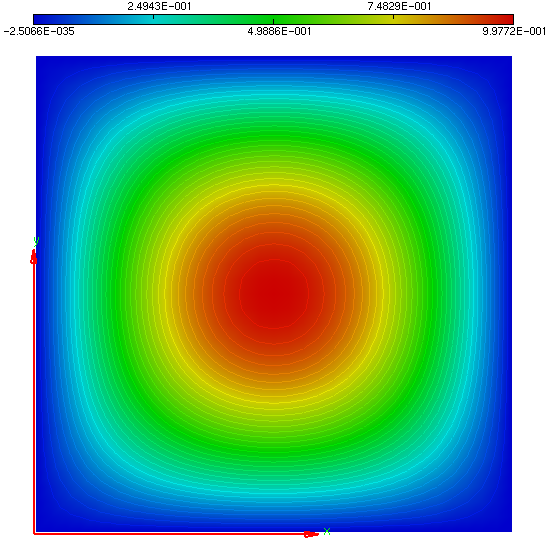
\includegraphics[width=\linewidth]{direct}
\end{figure}
Different cases of mesh size and time step length were studied to show the dependent of error on the mesh smoothness. We also use two different schemes
\begin{itemize}
	\item Backward Euler scheme
	\begin{figure}[h!]
		\centering
		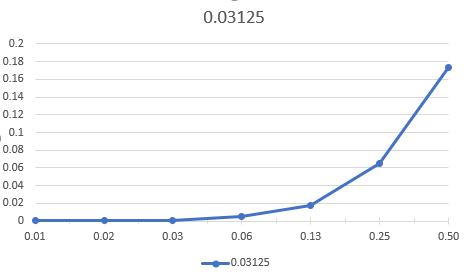
\includegraphics[width=\linewidth]{graph}
	\end{figure}
	\item Crank-Nicolson scheme
\end{itemize}
The approximate solution at final time is illustrated below.
\subsection{A problem of thermal engineering}
In the aspect of thermal engineering, the simulations of heat transfer attend in several applications. In [...] the author mentioned a realistic heat problem which can be solve by simulating the heat transfer process.\\
Assuming there are two types of material with different thermal conductivity and price. We would like to build a thermal resistance wall from composite plate of the two materials that provide optimal thermal resistance properties and satisfies economical conditions. Let $V$ is the total volume of the plate, $V_e$ and $V_c$ are the volume of expensive and cheap material respectively, then the ratio
$$
\mu = \dfrac{V_e}{V} = \dfrac{V_e}{V_c + V_e}
$$
is fixed. Consider a rectangular room $\Omega_r$ has the size $L_x \times L_y$. At the center of the left wall located a radiator that keep the local temperature at $T_r$, denote as $\Gamma_r$, otherwise as $\Gamma_\alpha$. The thermal flux through the walls is expected to be zero, equivalent to the Neumann boundary condition
$$
\dfrac{\partial u}{\partial n} = 0 \quad \text{on} \quad \Gamma_\alpha.
$$
The right corner of the room is where we place our composite thermal resistance plate. Let $\l_x$ is the width of the plate. The right wall is consider the heat source and gain the Dirichlet boundary condition
$$
u = u_{ext} \quad \text{on} \quad \Gamma_{ext}.
$$
Finally, let $\kappa_a, \kappa_c$ and $\kappa_e$ is correspondingly the thermal conductivity coefficient of air, our cheap and expensive material. Based on our goal of minimizing the temperature inside the room, the cost function can be formulated as follow
$$
J = \dfrac{1}{|\Omega_a|}\int_{0}^{T} \int_{\Omega_a} u dx 
$$
This problem belong to the set of shape optimization problems or more generally is an inverse heat problem. These kinds of problems take part in large amount of engineering applications. An approach is to solve as much acceptable input cases as possible then determine which one is the optimal solution. This way requires numerous computations.



% --------------------------------------------------------------------
\section{Conclusion}
% --------------------------------------------------------------------


% --------------------------------------------------------------------
% biblio
% --------------------------------------------------------------------
\bibliographystyle{plain}
\bibliography{references}{}
\vfill

\end{document}
